\documentclass[10pt,twoside,slovak,a4paper]{article}

\usepackage[slovak]{babel}
\usepackage[IL2]{fontenc}
\usepackage[utf8]{inputenc}
\usepackage{graphicx}
\usepackage{url} 
\usepackage{hyperref}
\usepackage{cite}

\graphicspath{ {./images/} }

\pagestyle{headings}

\title{Detekcia podvádzania v online multiplayer hrách\thanks{Semestrálny projekt v predmete Métody inžinierskej práce, akademický rok 2022/2023, vedenie: Igor Stupavský}}

\author{Tomáš Drga\\[2pt]
	{\small Slovenská technická univerzita v Bratislave}\\
	{\small Fakulta informatiky a informačných technológií}\\
	{\small \texttt{xdrga@stuba.sk}}
	}

\date{\small 10.10.2022}



\begin{document}

\maketitle

\begin{abstract}
Ako zvolenú tému som si vybral detekovanie podvodov v online hrách. O túto tématiku som sa zaujímal už aj v minulosti, a tak mi prišla aj ako vhodná téma pre moju semestrálnu prácu v predmete Métody inžinierskej práce. V tomto článku sa dozviete ako sa doposiaľ detekovali podvody v online hrách, a taktiež ako sa to zmenilo s príchodom nových technológií.
\end{abstract}


\section{Úvod}\label{uxfavod}

Podvody vo videohrách sú stále častejšie medzi bežnými hráčmi, rovnako
aj medzi profesionálnymi hráčmi, čo ovplyvňuje zážitok pre všetkých
hráčov. 

Cheaty sú často bežne a~ľahko dostupné. Ak by len 6\% hráčov
používalo cheaty pri videohrách, pravdepodobnosť že sa stretnete
s~cheaterom pri hre 5 na 5 je 42,7\%\cite{pravdepodobnost}. 

Ak majú hráči podozrenie, že ostatní hráči pri hraní podvádzajú, často sa presunú k~hraní iných hier alebo začnú sami podvádzať, čím sa vytvorí nekonečný kolobeh.


\section{História}

V tejto sekcií si povieme ako sa používal anticheat doteraz a prečo prišiel čas na zmenu. 

Anticheat fungoval pomerne jednoducho, nakoľko nebolo možné overiť či hráč naozaj podvádza v dôsledku nedostatku informácií zo servera. Nedostatok informacií si môžeme spojiť so zabezpečením hry. No keďže nie je dostatok informácií na odhalenie podvodov, museli herné spoločnsoti prísť s novými riešeniami, nakoľko prichádzali o veľké množstvo peňazí a hry strácali na popularite.

\newpage

\hypertarget{typy-cheatov}{%
\section{\texorpdfstring{Typy cheatov
}{Typy cheatov }}\label{typy-cheatov}}

Pri streleckých videohrách sa môžeme stretnúť rôznymi typmi použitia
cheatov, ktoré rôzne ovplyvňujú priebeh hry u~všetkých hráčov.

\hypertarget{mechanickuxe1-asistencia}{%
\subsection{Mechanická asistencia}\label{mechanickuxe1-asistencia}}

Najčastejším cheatom pri hraní streleckých hier je automatické
zameriavanie zbrane na hlavu protivníka. Tento typ podvádzania výrazne
zvýhodňuje hráčov, oproti tým, ktorí cheaty nepoužívajú.\cite{aim}

\hypertarget{asistencia-vedomostuxed-hruxe1ux10da}{%
\subsection{Asistencia vedomostí
hráča}\label{asistencia-vedomostuxed-hruxe1ux10da}}

Druhým častým podvodom v~hrách je získanie iných vedomostí oproti
ostatným hráčom. To sa odráža od princípu streleckých hier a~to je
eliminovať súpera. Tento druh cheatov dáva hráčom informácie
najčastejšie o presnej~polohe ostatných hráčov na mapách. Tieto cheaty
môžu mať rôzne podoby. 

Tento typ cheatov sa nazýva aj vizuálny hack,
alebo wallhack. To upravuje steny a~predmety vo videohrách a~ich
priehľadnosť, čím hráč môže vidieť ukrytého súpera. Taktiež je možná
úprava mapy, kde vidieť farebné odlíšenie spoluhráčov a~súperov.\cite{wallhack}

\hypertarget{asistencia-vedomostuxed-hruxe1ux10da}{%
\subsection{Motivácia pre tvorbu anticheatu}\label{asistencia-vedomostuxed-hruxe1ux10da}}
Aby sa cheatovaniu, tým pádom strate hráčov zabránilo, developeri
vytvárajú anti-cheat softvéry na detekciu cheatov ešte predtým ako sa
dostanú do hry.

Techniky data miningu analyzujú informácie v~dátach zariadenia na
zistenie cheatovacích softvérov. Táto technika však nie je ohľaduplná
k~súkromiu hráčov, nakoľko má anti-cheat softvér prístup ku všetkým
dátam hráča. Súkromnejšie techniky zistenia cheatov v~hrách momentálne
nie sú dostupné.
\newpage

\hypertarget{prieskum}{%
\section{\texorpdfstring{Prieskum podvádzania v hrách
}{Prieskum podvádzania v hrách}}\label{prieskum}}

Na svete neexistuje dostatok štúdií k tejto problematike no následujúce fakty sú sústredené na tri hlavné psychologické faktory. Súťažná motívacia, sebaúcta a agresia.

Agresia je dôležitý faktor, ktorý blízko súvisí so súťažnou motívaciou, a taktiež zvyšuje mieru podvádzania.

Sebaúcta znížila mieru podvádzania ale neovplyvnila súťažnú motívaciu. Nízka sebaúcta je spojená so správaním v realnom živote. Podľa štúdií ľudia s nízkou sebaúctou sú oveľa náklonnejší k podvádzaniu než tí, ktorí ju majú vysokú.\cite{pries}

V následujúcej tabuľke (Tabuľka~\ref{fig:mesh2}) môžeme vidieť najčastejšie druhy podvodov, a taktiež dôvody pre podvádzanie. Z údajov možno ľahko vyčítať, ktoré faktory najviac ovplyvňujú hráčov a prikláňajú ich k podvádzaniu.


\begin{table}[!ht]
    \centering
    \begin{tabular}{|l|l|l|l|l|}
    \hline
        Dôvody pre podvádzanie & ~ & Najčastejšie podvody & ~ & ~ \\ \hline
        ~ & ~ & ~ & ~ & ~ \\ \hline
        Frustrácia & 49\% & Wallhack & 37\% & ~ \\ \hline
        Pôžitok & 48\% & Aimbot & 30\% & ~ \\ \hline
        Udržať sa & 36\% & Ghosting & 24\% & ~ \\ \hline
        Poraziť & 35\% & Griefing & 22\% & ~ \\ \hline
        Financie & 33\% & Botting & 20\% & ~ \\ \hline
    \end{tabular}
    \caption{Prieskum dôvodov, pre ktoré hráči podvádzajú}
    \label{fig:mesh2}
\end{table}

\section{\texorpdfstring{Spôsoby zabránenia podvádzania v hrách
}{Spôsoby zabránenia podvádzania v hrách}\label{sposoby}}

V hernom priemysle existuje naneštastie veľa druhov podvodov, a tak nie je možné vytvoriť jedno univerzálne riešenie pre všetky podvody. 

Napríklad problém s Aimbotom alebo mechanickou asistenciou o ktorej sme sa bavili v časti~\ref{mechanickuxe1-asistencia} by sa dal vyriešiť prostredníctvom modelu, ktorý by kontroloval jednotlivé premenné hráča a zhodnotil by, či by ich vedel človek legitímne vykonať. Ak nie, je jasné, že sa jedná o podvodníka.

Ďalším príkladom podvodu je podvádzanie cez sieť pomocou umelého oneskorenia, ktorý spôsobí protivníkom dojem ako keby hráč zamrzol. Tento problém by sa dal vyriešiť dedikovanými servermi, pri ktorých by hráči nemali prístup k žiadným údajom a boli by len hostia. 

Ak porovnáme obe métody riešenia podvodov v hre a podvodov cez sieť, môžeme vidieť, že sú diametrálne odlišné, a tak nie je možné použiť len jedno univerzálne riešenie. Herné spoločnosti tak musia zabránit podvodom v hre, ako aj podvodom v sieti rozlišnými spôsobmi.\cite{solve}

\newpage


\section{Diagram aktivity}\label{uxfavod}

Diagram aktivity je jeden z UML diagramov, ktorý opisuje správanie. Tento diagram sa používa na modelovanie procedurálnej logiky, procesov a zachytenia workflow. Sekvenciu jednotlivých krokov v diagrame aktivít určuje riadiaci tok. Každý proces v diagrame aktivity je reprezentovaný sekvenciou jednotlivých krokov, ktoré sú v modeli zakreslené ako:

akcie – atomické ďalej nedeliteľné kroky


vnorené aktivity – volanie iných aktivít.

\begin{figure}[h]
    \centering
    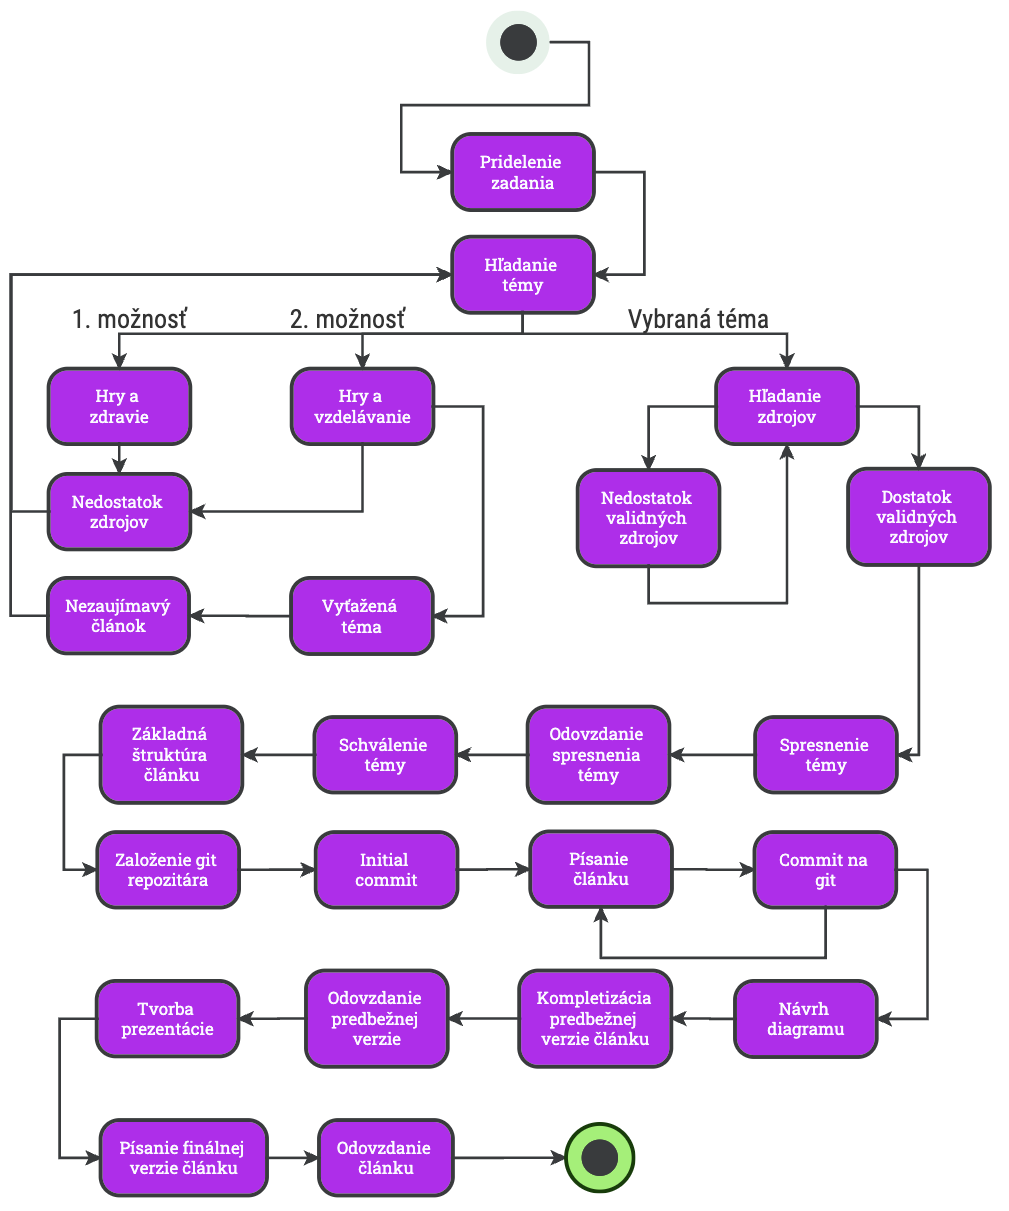
\includegraphics[scale = 0.65]{diagram.png}
    \caption{Diagram aktivity pre písanie článku}
    \label{fig:mesh1}
\end{figure}

Na obrázku (Obr.~\ref{fig:mesh1}) môžeme vidieť diagram aktivity podľa, ktorého som postupoval pri tvorbe článku. Diagramy sú dôležite pre vizuálizáciu práce a aj pre lepšie pochopenie. Viac o vizuálizácií sa môžete dozvedieť v časti ~\ref{viz}.

\newpage


\hypertarget{reakcia-na-prednasky}{%
\section{\texorpdfstring{Reakcia na prednášky
}{Reakcia na prednášky }}\label{reakcia-na-prednasky}}

V tejto časti článku sa pozrieme na určité témy z prednášok, ktoré pozitívným vplyvom oplyvnili moju tvorbu článku. Tieto témy boli pre mňa najprínosnejšie a ich využitie v praxi je enormné.
\hypertarget{git}{%
\subsection{Git}\label{git}}

Je systém, ktorý zabezpečuje kontrolu verzii. Používa sa primárne na verziovanie kódu. Je to užitočný nástroj, ktorý pomáha developerom s prehľadom ich kódu, a taktiež so zachovaním kódu. Git nám zabezpečuje, že náš kód sa nám nikdy nestratí a vždy zostane v bezpečí. To je dôležité hlavne pre veľké spoločnosti ale dokážeme z toho profitovať aj my. 

Git sme použili na verziovanie nášho článku. Hlavnou výhodou je zachovanie starších verzií. To v praxi znamená, že pokiaľ sme náš článok nejako zmenili ale neboli sme spokojný s výsledkom, mohli sme sa jednoducho vrátiť k našej pôvodnej verzií. 

Git je mocný a efektívny softvér, ktorý nám pomáha na každodennej báze s vývojom našich aplikácií a s verziovaním našich projektov. Dokážeme ho využiť prostredníctvom príkazového riadku. Ak nechceme využívať príkazový riadok môžeme využiť poskytovateľov hostingu pre Git ako je napríklad GitHub, Launchpad a GitLab.\cite{git}

\hypertarget{viz}{%
\subsection{Vizualizácia}\label{viz}}

V informatike je dôležitá pri vývoji hardvéru a softvéru. Slúži na reprezentáciu reality na inej úrovni, často takej, ktoré je zrozumiteľnejšia pre bežného človeka. Najčastejšie sa pre softvérové riešenia vytvárajú diagramy. 

Diagramy môžu mať rôzne podoby, ale pre informatiku sú veľmi dôležité tie v tvare grafov - uzly spojené hranami. Dôležité je uvedenie a spojenie uzlov, nie ich exaktné usporiadanie a veľkosť ako napr. v technickom kreslení. Uzly môžu znázorňovať štrukturálne jednotky alebo jednotky správania. Hrany pritom označujú vzťahy medzi štrukturálnymi jednotkami alebo toky údajov a riadenia. Textové označenie uzlov a hrán - aj pri grafickom vyjadrení.\cite{viz}

\hypertarget{scrum}{%
\subsection{Scrum}\label{scrum}}

Je systém pre riadenie projektov s dôrazom na vývoj softvéru. Používa aj v iných oblastiach vrátane výskumu, predaja a pokročilých technológií. 

Jeho základom je rozdelenie práce v tíme na menšie kusy, ktoré je možné dokončiť v istom časovom okne. Scrum tím hodnotí pokrok na každodenných stretnutiach, ktoré sa nazývajú denné Scrum Meetings. 

Na konci tím usporiada dve ďalšie stretnutia.  Jedno určené na demonštráciu práce pre klienta.  Cieľom druhého je umožniť tímu reflektovať a zlepšovať sa.\cite{scrum}
\newpage

\section{\texorpdfstring{Záver
}{Záver}\label{zaver}}

V článku sme sa dozvedeli prečo je dôležité zabrániť podvádzaniu v online multiplayer hrách. Pravdepodobnosť, že sa stretnete s cheaterom je takmer 40\%.

Spomenuli sme rôzne spôsoby akými sa cheaty odhaľujú, a taktiež základné druhy cheatov, ktoré sú používané najčastejšie.

Na základe prieskumu sme sa dozvedeli, ktoré faktory najviac ovplyvňujú hráčov a privádzajú ich k podvodom.

Uviedli sme základnú logiku pre riešenie problémov s podvádzaním a bližšie sa pozreli na dva hlavné druhy riešenia podvodov.

Ukázali sme dôležitosť vizuálizácie pri práci s technológiami, a taktiež sme priblížili čo sú UML diagramy.

A ako posledné sme spomenuli to najdôležitejšie a najužitočnejšie z prednášok na predmete Metódy inžinierskej práce.

\newpage


\bibliography{literature}
\bibliographystyle{ieeetr}
\end{document}